\section{Irradiation at the Rhode Island Nuclear Science Center}
\label{sec:irradiation}

\subsection{Rhode Island Nuclear Reactor}
\label{subsec:RINSC}
The Rhode Island Nuclear Science Center (RINSC) houses a \SI{2}{\mega\watt}, light-water cooled, pool-type reactor in Narragansett, Rhode Island, USA.
Its core consists of fuel assemblies reflected with a combination of graphite and beryllium.
The fuel is plate type U$_3$Si$_2$ cladded with aluminum enriched to less than 20$~\%$ Uranium-235.
In general, there are six different methods to irradiate materials at RINSC.
However, only the delivery method via the beam port was applicable because it is the only sample delivery system large enough to accept full-sized HGCAL silicon sensors.
The beam port in question had not previously been used for experiments, only for facility-related work.
A sketch of the beam port and a photo of its inside are shown in \ref{fig:beam port_Schematic}a and b.
\begin{figure}
  \begin{center}
    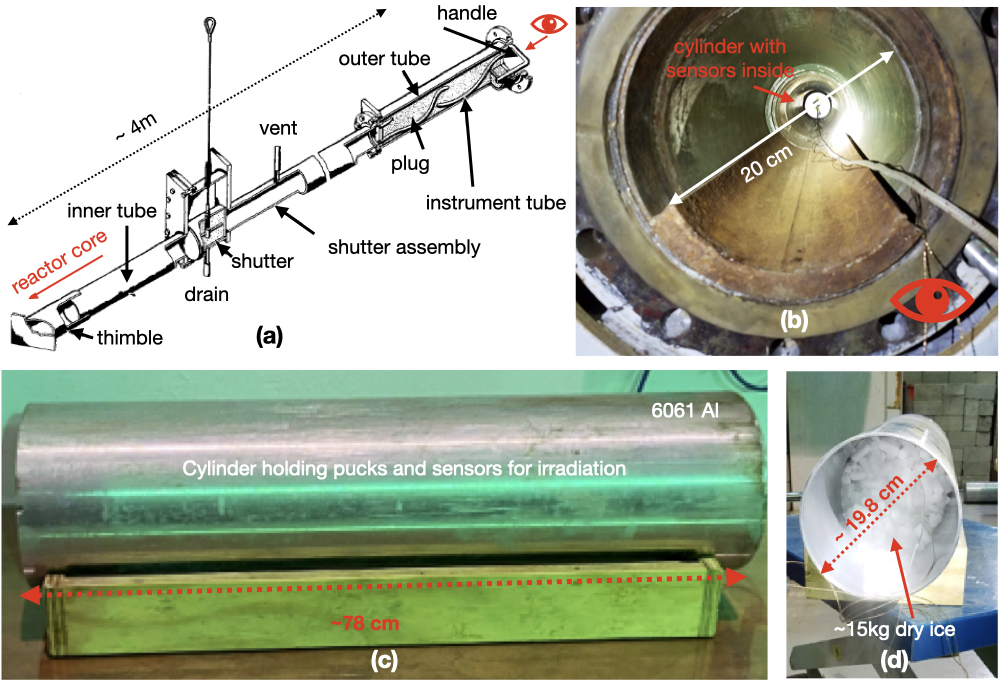
\includegraphics[width=0.99\textwidth]{figures/figures_edited_001.jpeg}
    \caption{(a) Schematic of the beam port sample delivery system at RINSC.
    (b) The view down into the beam port used for these irradiation studies.
    (c) The sample delivery cylinder that contains the sensor-holding hockey pucks and (d) dry ice for cooling of the silicon sensors in the beam port during and after irradiation.
    }
    \label{fig:Beamport_Schematic}
  \end{center}
\end{figure}
It measures about \SI{4}{\metre} from its opening to the termination near to the reactor core, and it can accommodate samples with diameters of up to \SI{20}{\centi\metre} and with depths up to \SI{90}{\centi\metre}.
A shutter assembly is located \SI{3}{\metre} from the opening of the beam port, which must be raised to allow for the insertion of the samples and closed prior to the start of the reactor.
A \SI{85}{\centi\metre}-long lead plug serves as a radiation shield that has to be inserted into the opening of the beam port prior to the start of the irradiation.

\subsection{Irradiation of HGCAL silicon sensor prototypes}
\label{subsec:irradiation}
Given the constraints of the beam port system at RINSC, a dedicated sample delivery method had to be developed for irradiating HGCAL silicon sensors.
This new sample delivery allows for:
\begin{itemize}
  \item Positioning sensors as close to the reactor core as possible,
  \item protecting them from physical damage during the loading, irradiation, and unloading,
  \item keeping the irradiated sensors at cold temperatures during and after the irradiation,
  \item monitoring the temperature of the samples inside the beam port.
\end{itemize}
Two compatible pieces of hardware were manufactured for the irradiation of the HGCAL silicon sensor prototypes: a sensor container, referred to as a "hockey puck", and a sample delivery cylinder (see~\ref{fig:Beamport_Schematic}c). 
The former is used to protect, orient, and store the sensors during irradiation while the latter is used to protect and locate the hockey puck inside the beam port.
The cylinder is made from 6061 aluminum, has an outer diameter of \SI{19.8}{\centi\metre} fitting into the beam port, and the inner diameter of the cylinder is \SI{19.1}{\centi\metre} allowing for smooth insertion and removal of the hockey pucks.
%Recommendation by Timo: Unnecessary detail to be removed
%The cylinder has a welded cap on the end that faces the reactor core, and a removable cap with threaded holes for 8 - 32 countersunk flat head machine screws that are flush with the outer wall of the cylinder. 
%Both the welded cap and the removable cap have vent holes to allow for air to flow into and out of the cylinder.
%An eye bolt is screwed into the removable cap to facilitate removing the cylinder from the beam port after irradiations.
Three different hockey puck materials were considered, see~\ref{fig:Pucks_Arrayed}a: Oak, acrylic, and PEEK. 
Those differ in their mechanical properties with respect to temperature and humidity fluctuations, in their activations, radiation hardness and overall cost.
As practical compromise between these factors, acrylic was found most suitable for irradiation up to fluences of $5\cdot 10^{15}\neqcm$, and PEEK material suitable for higher fluences. 
The usage of oak was discarded because of its unfavorable tendency to absorb moisture.
\begin{figure}
  \begin{center}
    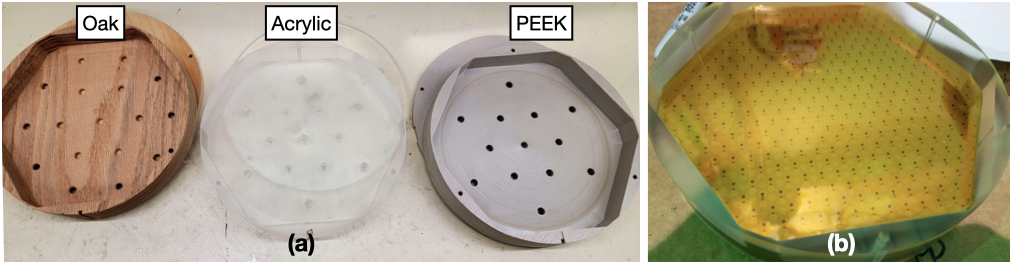
\includegraphics[width=0.99\textwidth]{figures/figures_edited_002.jpeg}
    \caption{(a) Sample containers ('hockey pucks') designed to hold HGCAL silicon sensors for neutron irradiation at RINSC. 
    Wood (oak), acrylic, and PEEK were the puck materials that were experimented with.
    (b) An 8'' high-density HGCAL prototype silicon sensor inside an acrylic puck covered with a Kapton\texttrademark$~$foil.}
    \label{fig:Pucks_Arrayed}
  \end{center}
\end{figure}
The puck base has an outer diameter of \SI{18.6}{\centi\metre} that allows for a smooth fit inside the cylinder. 
The interior of the puck is milled out in the profile of the silicon sensors with an additional clearance of \SI{1}{\milli\metre}. 
With these constraints the thinnest sections of the wall of the puck are slightly over \SI{1}{\milli\metre} thick which provides a difficult machining challenge.
%Recommendation by Timo: Unnecessary detail to be removed
%The puck has a lid, made from the same material as the base, that matches the outer diameter of the base and provides a way to close the puck during handling.
%Matching through holes in the base and lid allow for using nylon threaded rods and nuts to fasten the puck together. 
Kapton\texttrademark$~$foils were used to separate sensors in a stack such that no sensors are in direct contact with any metallic surfaces (cf.~\ref{fig:Pucks_Arrayed}b).
In addition, antistatic foam was used for covering the top and bottom of the sensor-Kapton\texttrademark$~$stack serving as a cushion  against the walls inside the puck.
%Sensors were irradiated in batches of four, which required ten layers of Kapton\texttrademark$~$foils and three to four layers of antistatic foam. 
After preparation of the puck, the latter was inserted into the delivery cylinder.
In general, the silicon sensors should be kept at low temperatures during the irradiation in order to limit unwanted thermal annealing.
For this purpose, the rest of the delivery cylinder was filled with 15-\SI{18}{\kilo\gram} of dry ice.
In order to monitor the temperature, PT1000 resistance temperature detectors (RTD) were inserted into the puck, at the front and back faces, to record the temperature throughout the irradiation for assessment of the expected sensor annealing during irradiation. 
%Before the cylinder was closed, the RTD wires were routed through the vent holes in the removable cap, and were connected to a dedicated temperature readout system outside the beam port.
%Recommendation by Timo: Unnecessary detail to be removed
%Once the cylinder had been fully packed, it was loaded onto a sled and inserted into the opening of the beam port.
%It was then pushed all the way inside, the shutter was lowered, the lead plug was inserted into the opening of the beam port, and the setup was ready for irradiation.
Representative temperature recordings from two irradiation rounds of different duration are shown in~\ref{fig:Round_10_Temperature_Profile}.
\begin{figure}
  \begin{center}
    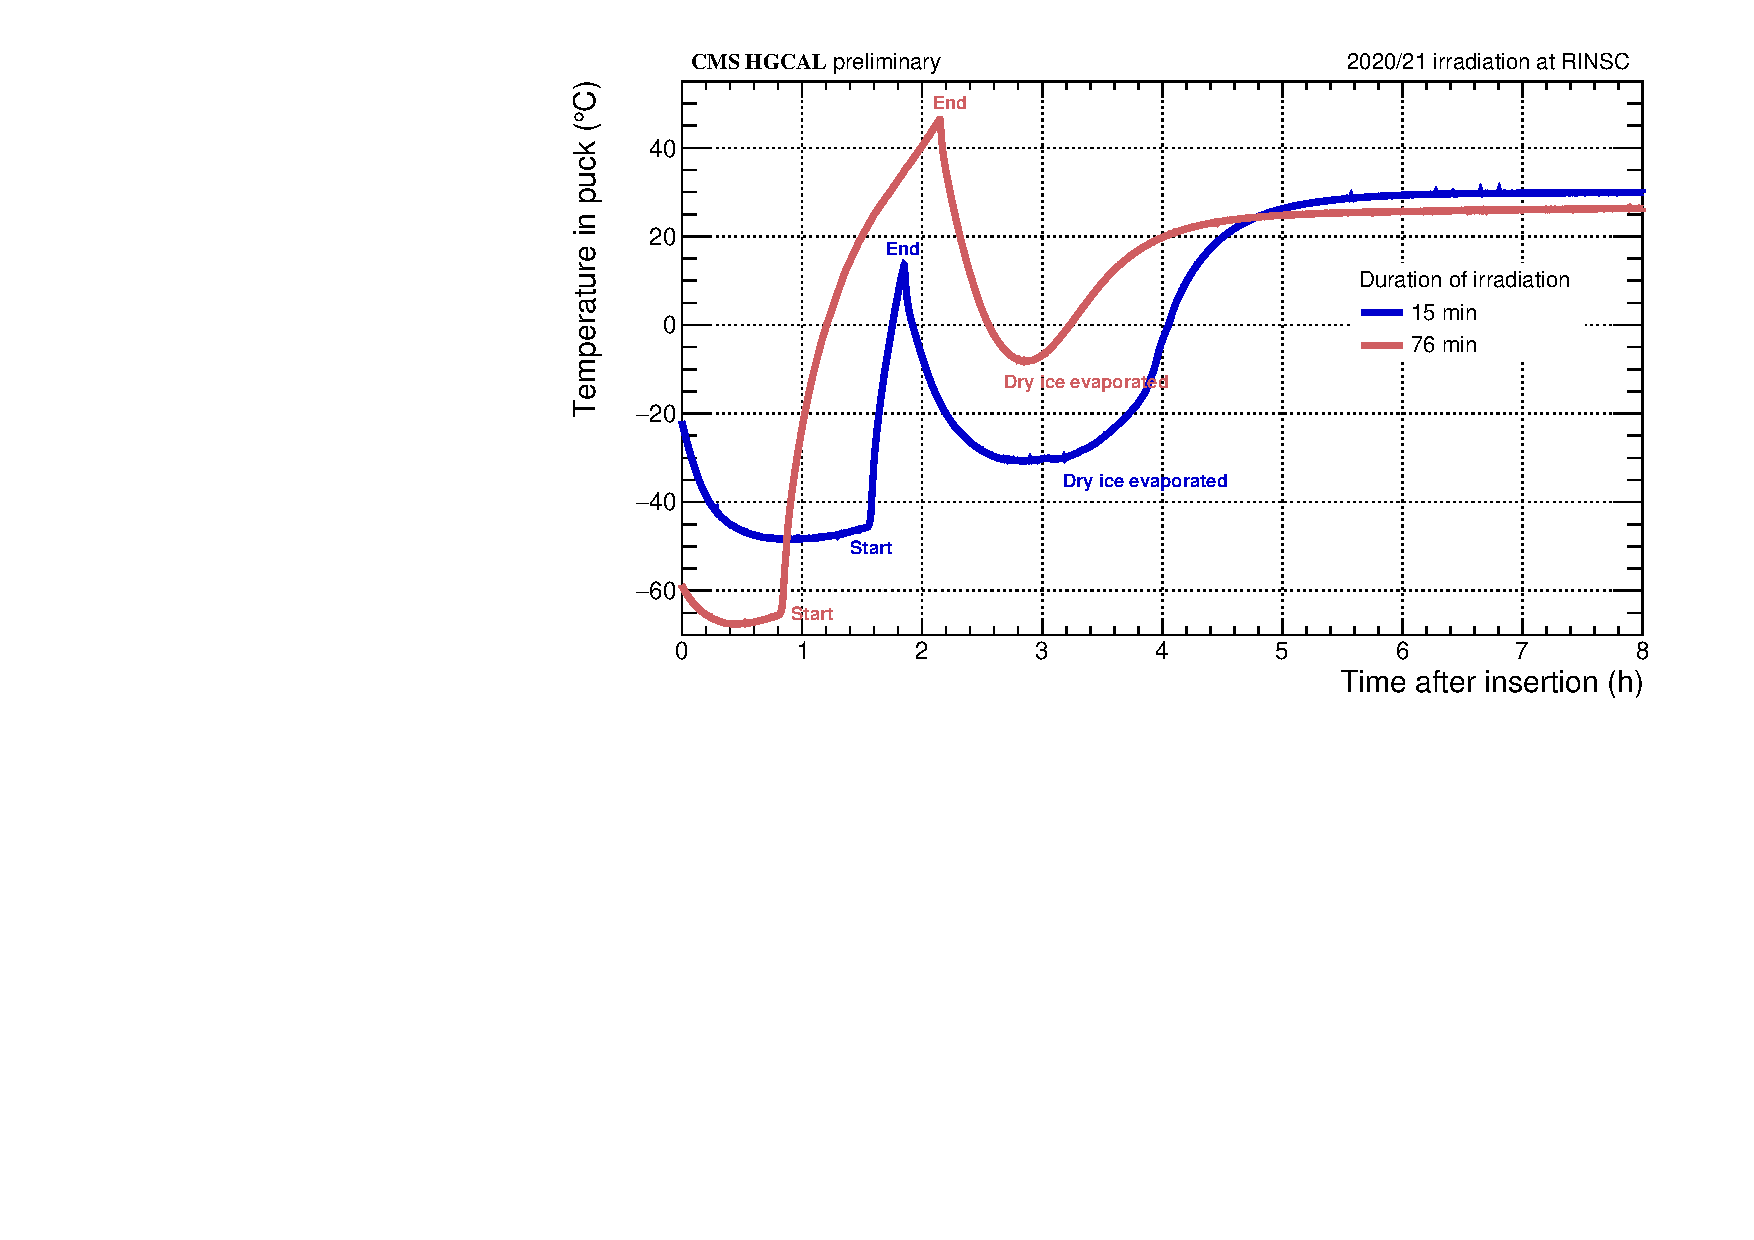
\includegraphics[width=0.69\textwidth]{plots/RINSC_temp/RINSC_temp.pdf}
    \caption{Representative temperature recordings during two of the RINSC irradiation rounds of HGCAL prototype silicon sensors. 
    The time when the irradiation was started and when it ended is indicated.
    The increase of the temperature towards its plateau coincides with the sublimation of the dry ice inside the delivery cylinder.
    }
    \label{fig:Round_10_Temperature_Profile}
  \end{center}
\end{figure}
During irradiation, the temperature rises significantly eventually reaching temperatures ranging from of a few \SI{10}{\celsius} to \SI{100}{\celsius}.
In fact, it was found that most of the dry ice eventually sublimated hereby.
Only after shutdown of the reactor, the temperature decreased again.
As a result, the annealing of the silicon sensors inside the beam port was not negligible.
The corresponding annealing time at \SI{60}{\celsius} varied between a few minutes to a few hundred minutes for all the HGCAL silicon sensors irradiated at RINSC in 2020/21 up to $\sim 10^{16}~\neqcm$.
After \SI{24}{\hour} in the beam port after irradiation, the cylinder's radioactive levels have decayed sufficiently such that it could be safely extracted and transferred into a storage freezer.

\subsection{Fluence Assessment}
In addition to the sensors, mechanical packing material, and temperature sensors, each puck contained a number of reference samples for measuring the fluence achieved during an irradiation round. 
Two different objects were found appropriate for measuring the fluences during this campaign: reference silicon diodes from the D0 experiment and ultrapure iron foils. 
The diodes were included inside the puck as close to the sensors as possible by encasing them in small plastic bags and taping them to the inside faces of the puck. 
By contrast, the iron foils were attached to the exterior of the cylinder for ease of removal and rapid counting. 
After irradiation, gamma spectra of the iron foils were measured at RINSC for derivation of the integrated fluence.
In addition, CV and IV measurements of the irradiated diodes were performed at Brown University to assess the depletion voltage, the associated dark current and ultimately the fluence assuming the literature value for the current-related leakage current rate of $\left(3.99\pm 0.03\right)\cdot 10^{-17}~$A/cm at \SI{20}{\celsius}~\cite{moll:SiDamages}.
%It was found empirically that the usage of commercially-available pin diodes saturated already at low fluences (below 4E14) and thus were not found to be particularly useful. 
The reference silicon diodes are most useful for the lower to medium range of the targeted fluences,  where their depletion voltage was well within the measurement range ($<\SI{1000}{\volt}$).
For higher fluences, full depletion of the silicon diodes could not be reached, and the gamma ray spectra derived from the iron foils are considered more reliable.
\ref{table:irrads} in~\ref{appendix:irrad_rounds} shows the estimated actual fluences from those reference samples.
In order to improve the accuracy of the fluence assessment, future irradiation of HGCAL silicon sensors at RINSC will include iron foils inside the puck as well as additional silicon test structures.